\documentclass[12pt]{article}

% PACKAGES

\usepackage{amsmath}
\usepackage{fancyvrb}
\usepackage{hyperref}
\usepackage{multicol}
\usepackage{wrapfig}
\usepackage{tikz}
\usepackage{graphicx}
\graphicspath{ {./images/} }

\usetikzlibrary{shapes.geometric, arrows}

% CUSTOM COMMANDS

\newcommand{\row}[1]{\texttt{#1}}
\newcommand{\br}[0]{\vspace{10pt} \noindent}
\newcommand{\footurl}[1]{\footnote{\url{#1}}}
\newcommand{\nth}[2]{#1\textsuperscript{#2}}

% TITLE

\title{Designing and prototyping a visual, incremental composing tool for change ringing}
\author{Benjamin White-Horne \\ \emph{University of Oxford,} \\ \emph{Department of Computer Science}}



\begin{document}

\maketitle



\pagebreak

\section*{Abstract}

This project concerns the designing and prototyping of Jigsaw, an application to aid church
bell-ringing composers.  Jigsaw aims to be for bell-ringing composers what Microsoft Word is for
writers.

Change ringing is where a team of people ring a set of 6--12 church bells in continually evolving and
pre-determined sequences. The art of composing concerns designing these sequences for ringers to
perform and dates from the 1700s.  Composing was traditionally done by hand, and there are some
computer tools to automate parts of the process. Jigsaw breaks new ground and, as far as the author
is aware, is the first graphical, user-friendly and intuitive tool to aid the composer.

Jigsaw has an innovative graphical interface to make composing easier, more intuitive and more
accessible for beginners. The tool was designed to a general goal and specific requirements, and was
beta-tested by experienced composers to gain feedback and improve the design.

Jigsaw is deployed as a static web app using GitHub pages.

The project also created BellFrame, a fast and idiomatic Rust library which provides easy-to-use
data types for ubiquitous concepts in change ringing. BellFrame has good documentation with code
examples. In the next stage of development, once its API is more stable, it will be published to
Rust's package repository for general use.



\pagebreak

\tableofcontents



\pagebreak

\section{Introduction}

\subsection{Project Goals}\label{sec:design-goals}

This project concerns prototyping an application to \emph{aid} composers whilst requiring the
smallest possible change to their existing workflow.  This is analogous to what Microsoft Word
provides for writers --- a kind of `automated paper' which automatically annotates your work with
data that is tedious to compute manually whilst still providing it in a format that you are familiar
with (i.e.\ words on a page).  Additionally, it must provide correct feedback regardless of the
completeness of the composition.

\subsection{Specific Requirements}\label{sec:requirements}

Whilst the goal above gives a general design direction, more specific requirements are needed to
build a cohesive application.  Therefore, I split this general goal into five specific goals which
were used to design and then assess the prototype application.  These goals were derived from
observing the limitations of existing tools, conversations with well-known composers, and experience
gained from experimentation early in the project.  

\paragraph{Ease of Use} The application should be graphical and present its data in a way that is
intuitive and accessible to the user.  It should also be made so that anyone can install and use it
easily, without any technological knowledge or a lengthy installation process.

\paragraph{Completeness} There is a concrete definition of what is considered `Change
Ringing', and the states representable in the application must be a superset of those allowed by
this definition.  This definition is provided by the Framework for Method
Ringing\footurl{https://cccbr.github.io/method_ringing_framework/classification.html}.
\paragraph{Incremental} The application should allow the user to incrementally build up their
composition, in whatever order they want, starting wherever they want to.  Specifically, it must
be able to represent `partial' compositions --- i.e.\ a set of composition `fragments' which will
eventually be combined into a full composition.

\paragraph{Instant} Feedback on important measures like truth, music content and length should
update instantly whenever the composer changes their composition.  

\paragraph{Visual} Everything that can be understood visually should be displayed visually.  Where
specific numerical data is required (e.g.\ length), these should also be provided in a suitable
format.

\subsection{Jigsaw}

\subsubsection{Overview}

The application I designed and prototyped for this project is called Jigsaw.  The GUI has two main
parts: an infinitely scrollable canvas where the composition fragments are, and a folding sidebar
which overlays the canvas and shows information that cannot be represented in the canvas.  Jigsaw is
intended to be used on a desktop with a keyboard and mouse.

Jigsaw supports a large number of operations to modify partial compositions.  All of these are bound
to keys on the left side of the keyboard (because the user's right hand is expected to be on the
mouse), and for consistency they apply their effects to the location of the cursor.

\subsubsection{Static Web Application}

Jigsaw is built to be run as a single static web page (i.e.\ it is a fixed set of files that can be
served by a simple HTTP server).  Releasing applications as static websites has many advantages:

\begin{enumerate}
    \item There is no start-up time for a new user --- they open the page in any browser and the
        application starts immediately.
    \item HTML canvas rendering (while extremely inefficient compared to OpenGL or Vulkan) is easy,
        fast enough to feel instant and looks consistently good across all browsers and operating
        systems.

        These performance concerns turned out to be a non-issue; after implementing simple culling
        of off-screen rows, there have been no issues with rendering performance when running on
        modern hardware.  Additionally, there are many opportunities to optimise the rendering if
        required, meaning that this will still be an easily fixable issue in the future.
    \item Having no dependence on a server both obviates the need for the user to make an account
        (which worsens the user experience) and also means that it can be deployed using GitHub
        pages or a similar service.
\end{enumerate}

Persistent storage is a challenge of static web applications, since websites cannot directly access
the file system for security reasons.  Cookies are one possible option but they are sent over the
network with every request, making them unsuitable for storing large amounts of data.  Browsers do
provide a persistent cache for network requests which can be arbitrarily read from and written to,
thus providing persistent storage.

\subsubsection{JavaScript and Rust/WebAssembly}

For Jigsaw's user interface, the native web languages (JavaScript, HTML and CSS) are the obvious
choice.  The `back-end' of Jigsaw, however, has to do a lot of complex operations on data every time
the user changes the composition being displayed.  This must be done quickly enough that the user
cannot perceive the delay, and must be reliable.

JavaScript is very unsuitable for this kind of workload.  Firstly, it has no static analysis, making
it unnecessarily difficult to write complex code correctly.  It also gives no control over memory
layout and is absolutely reliant on a JIT (Just In Time) compiler for performance.  Jigsaw's compute
pipeline consists of several thousand lines of code, which is unlikely to all be compiled by the JIT
compiler.


Therefore, another language is required.  Jigsaw's back-end is written in Rust, a systems
programming language which emphasises performance and safety (the two things Jigsaw needs).  The
Rust code is compiled to WebAssembly so it can run natively in the browser.  Other languages could
work for this purpose (for example TypeScript, C/C++ or Go) but I chose Rust for the following
reasons:

\begin{enumerate}
    \item Rust provides direct control over memory layout and has no garbage collector, providing
        consistently excellent performance when manipulating complex data structures.  The
        performance of TypeScript, for instance, is by definition no better than that of JavaScript.
    \item The Rust compiler performs a large amount of strict compile-time correctness checks on
        your code (including guaranteeing memory safety), making it easy to implement complex
        algorithms in ways that you know is correct and fast.  C/C++ and Go cannot compete in this
        regard.
    \item Rust has first class support for WebAssembly.  Jigsaw is greatly aided by
        \verb|wasm_bindgen|, which automatically generates binding code between native Rust and
        native JavaScript to let the two languages interface seamlessly.
    \item I am already proficient in Rust, so no time will be spent learning new languages for the
        project.
\end{enumerate}

\subsection{BellFrame}

When implementing Jigsaw, it became clear that a large amount of the Rust code was providing data
structures that were specific to change ringing but not just to Jigsaw.  Therefore, it made sense to
keep this code separate as a stand-alone library (named BellFrame) that could be re-used in other
ringing-related projects.  I made sure that BellFrame has good documentation and test coverage, and
I will publish it to Rust's package repository once its API becomes more stable.  Despite not being
an explicit goal of this project, BellFrame is as much a product as Jigsaw itself.



\pagebreak

\section{Overview of Change Ringing}

\subsection{Background}

Change ringing is a niche and not well-understood activity so this section will serve as a short
introduction to the topic and overview of the aspects of change ringing which are relevant to this
project.  A more complete overview can be found on
Wikipedia \footurl{https://en.wikipedia.org/wiki/Change_ringing}.  I have also provided a glossary of
commonly used terms in Section~\ref{sec:glossary}.

Change ringing (sometimes known as full-circle church bell ringing) originated in English
churches in around 1600, where churches began hanging sets of tuned bells on wheels in towers.
The installations range from 3 to 16 bells, with even numbers from 6 to 12 being almost ubiquitous.
These bells are typically quite heavy (bells over a ton are fairly common) and are spun
back and forth through 360 degrees like a pendulum.  All the bells are rung once in a sequence which
changes each time.  A piece of change ringing is a sequence of permutations, known as `changes'
(hence `change ringing').  Because ringers have little control over the frequency of their bell,
bells only move by at most one place between two adjacent rows.  On paper, we write these
permutations in order as rows of numbers and by convention, the bells are numbered sequentially with
`1' referring to the highest-pitched bell in the tower.  For example:

\begin{verbatim}
12345678
21436587
12463857
21648375
  ...
\end{verbatim}

In order to break up the walls of numbers, we will often draw coloured lines through the path of
some bells.  By far the most common is to give the highest pitched bell (the `1') a thin red line,
and the lowest pitched bell a thick blue line (this is used extensively in the diagrams throughout
this report --- see Figure~\ref{fig:little-bob} for a simple example).  

\subsection{Methods}

A performance of ringing will often contain thousands of individual rows.  Physical aids to memory
are not permitted during performances so the ringers must ring thousands of unique rows completely
from memory.  Memorising them all directly is clearly not feasible, so compositions are built up
from repeating patterns known as `methods'.

A method has a name (often with historical or geographical connections). In the method each bell
moves through a pre-determined path, moving back and forth within the sequence. Ringers learn these
paths to help them remember where to ring in the sequence of rows.

A single instance of a method is called a `lead' and can be thought of as a super-permutation; it
takes a start row and produces a sequence of rows, ending with the row which the next lead should be
started (rows like this are not considered part of the super-permutation).  This final row is
considered part of the next lead, and is usually shown greyed out to emphasise this.

\begin{figure}[h!]
    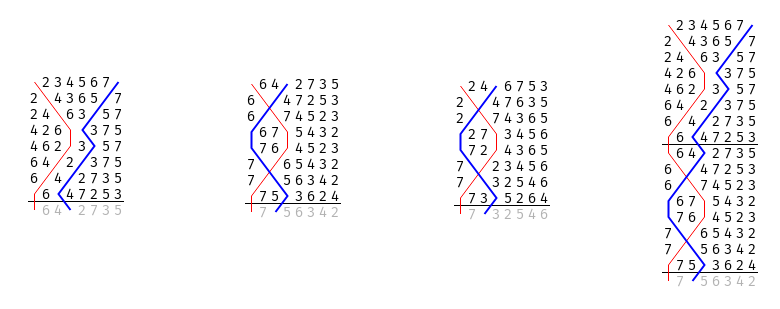
\includegraphics[width=\textwidth]{lb8}
    \caption{A collection of leads of the same method.  Note the use of lines to represent the
    paths of bells 1 and 8.}\label{fig:little-bob}
\end{figure}

For example, the left three columns shown in Figure~\ref{fig:little-bob} are all leads of the same
method (this particular method is known as `Little Bob Major').  The second lead starts with the
`leftover' row of the first, and therefore they can be concatenated to form the fourth column.

Note that a single lead of this method preserves the location of the bell at the start of the
row.  This is an extremely common feature of methods because it allows ringers to orient
themselves around this `fixed' bell and therefore helps prevent mistakes.

\subsection{Compositions}

A `composition' is a sequence of rows of some length which satisfies the adjacency property and
starts and finishes with the row containing bells in descending order (\row{123456\ldots}, known as
`rounds').  Thus, the above diagram shows a valid composition.

The task of a composer is to create compositions which have some set of desirable features (which is
likely to depend heavily on the circumstances of each performance).  In order to understand the
rationale behind this project and gauge its success, we must first understand some of the most
important features or constraints of compositions.

\subsection{Features of Compositions}

\subsubsection{Stage}

The ``stage'' of a composition refers to the number of bells which it uses.  These are given
specific names (for example ``Triples'' refers to 7 bells and ``Major'' refers to 8 bells), but
these are confusing and are outside the scope of this report.

Since towers almost always contain an even number of bells, the stage of a composition is not
necessarily the number of bells that the composition is rung on.  For example, compositions of
``Triples'' are almost ubiquitously rung on 8 bells with the lowest bell always remaining at the end
of each row (this is known as a ``cover bell'').

\subsubsection{Truth/Falseness}

For a given stage $n$, there are $n!$ possible rows that a composition of that stage can use.  If we
were to count the number of occurrences of each row in a composition, then the composition is
``true'' if these counts are as balanced as possible.  If a true composition on stage $s$ contains
$n$ rows, every possible row must be repeated either $\left\lfloor \frac{s}{n!} \right\rfloor$ or
$\left\lceil \frac{s}{n!} \right\rceil$ times.

For example, imagine a composition of 1260 rows on 5 bells.  There are $5! = 120$ possible rows so
for this composition to be true, every row must be repeated at least 10 times and 60 of these must
be repeated 11 times.

Because $n!$ quickly gets huge as $n$ grows, a very common case is where $s < n!$. In this case
$\left\lfloor \frac{s}{n!} \right\rfloor = 0$ and $\left\lceil \frac{s}{n!} \right\rceil = 1$ so
for these compositions, ``truth'' is equivalent to the rows being unique.

It is worth noting here that compositions are written with rounds at both the start and end.
However, when discerning truth these are only counted once --- otherwise, nearly every composition
would be false.

\subsubsection{Length}

The `length' of a composition is the number of rows which it contains.  Like falseness, external
rounds is only considered once.

96.5\% of performances and 90.5\% of compositions\footnote{There have been 136,206 performances of
peals and 312,004 of quarter peals (out of 464,564 total).  There are 31,827 published peal
compositions and 8,597 quarter peal compositions (out of 44,676 total).  Statistics were taken from
BellBoard (\url{bb.ringingworld.co.uk}) and Composition Library (\url{complib.org}) on \nth{23}{rd}
of May 2021.} have one of two length ranges:

\begin{enumerate}
    \item A \textbf{Peal} consists of at least 5000 rows (about 3 hours' ringing).
        The number 5000 is chosen because historically the pinnacle of ringing challenge was to ring
        every permutation of 7 bells, which results in $7! = 5040$ rows.  This was recently rounded
        down to 5000 for all numbers of bells, but the majority of people prefer the completeness of
        5040 rows for peals of 5, 6 or 7 bells (where every possible row is rung the same number of
        times).
    \item A \textbf{Quarter Peal} consists of at least 1250 rows (a quarter of a peal's length, and
        about 45 minutes' ringing).  Due to the reduced completion time, these are much more
        common than peals.  Half peals ($\ge 2500$ rows) and double-length peals ($\ge 10,000$ rows)
        are both recognised lengths but performances of them are very rare.
\end{enumerate}

Half peals ($\ge$ 2500 rows) and double-length peals ($\ge$ 10,000 rows) are also recognised lengths
but performances of them are very rare.

Also, every row above the lower bound is extra ringing time for little gain in performance merit,
and therefore composers try to make compositions which are as close as possible in length to these
lower bounds.  Indeed, lengths within the ranges $1250 \le l < 1300$ or $5000 \le l < 5100$ are
almost ubiquitous.

\subsubsection{Music}

If we are composing for $\ge 8$ bells, then our composition will not contain every possible row and
we therefore have the opportunity to decide which rows get included and which do not.  Of these, some
may be more favourable or ``musical'' than others.

Ringers like rows which start or finish with at least 4 consecutive bells, which give a pleasing
musical effect.  The exact bells are usually unimportant and the longer the run the better.  For
example \row{34567812} starts with a descending run of 6 bells, and is therefore preferable to
\row{57864321} which ends with an ascending run of 4 bells.  Both of these are preferable to
\row{18346527} which has no runs.

\subsubsection{Complexity}

Complexity does not have a clear mathematical definition and therefore this project will make no
attempt to automate it.  However, it is still an important concept which roughly corresponds to how
repetitive and predictable the composition is.

In general, we want to make these things as simple as possible because that will open your
composition to be performed by more people.  However, sometimes \emph{the point} of a composition is
to be a challenge for the ringers, in which case complexity is a target not a limitation.

\subsubsection{Multi-Part Compositions}

Because repetitive compositions are easier to learn, it is very common to create which have multiple
`parts'.  In this case, a part of a composition is a chunk which, when repeated end-to-end, produces
a full composition.  This is clearly an advantage since, if a composition has $n$ parts, a potential
conductor only needs to learn \nth{$\frac{1}{n}$}{th} of the composition and repeat it multiple
times.

Each `part' will not end in rounds and therefore is not a composition itself.  A common way to
create multi-parts is to rotate bells 2, 3 and 4 to give 3 parts.  In writing this would look like
Figure~\ref{fig:multi-part}.

\begin{figure}
    \centering
    \begin{BVerbatim}
12345678
 <part>
--------
13425678
 <part>
--------
14235678
 <part>
--------
14235678
    \end{BVerbatim}
    \caption{An example of a 3-part composition.}\label{fig:multi-part}
\end{figure}

\subsubsection{Summary}

In general, stage, length and falseness are hard constraints which composers have little choice over
and must work around.  Most of the time, the composer fixes some target level of complexity and
tries to get as much music or interest as possible within that constraint.  Also, many composers
make compositions that they intend to conduct themselves, allowing for a higher level of complexity
because they already have an intimate knowledge of the composition before learning it.



\pagebreak

\section{Design}

\subsection{Process}

When starting to design Jigsaw I had a rough sketch of what the application would look like (for
example, I knew I wanted to embed composition fragments into an infinite canvas).  I then refined my
rough ideas into the specific requirements enumerated in Section~\ref{sec:requirements}.

At each point in the development process, I would pick the goal that has the least dependence on
goals or code which I had not completed.  Care was taken to move on to new goals instead of fixating
on one part of the design, since often improving other parts of the design provides additional
context that affects already existing changes.  This creates an overall more cohesive design, as
well as preventing the project from stalling over small design problems.

For example, the first goal I worked on after writing some necessary utility code was the visual
aspect of rendering fragments --- because regardless of future decisions, Jigsaw has to have be able
to render fragments nicely in order to satisfy the goals.

On the most part, this ordering was quite obvious, but there were a few cases where the I approached
problems in what turned out to be the wrong order.  This did not detriment the resulting design ---
it just meant that some features took longer than necessary to implement.  In particular, lead
folding was implemented late in development and required radical changes to the Jigsaw's internal
pipeline.  A large amount of time would have been saved by implementing it earlier in the design
process.  

From a design perspective, this approach worked well --- Jigsaw's design is quite consistent and
intuitive and I am pleased with the result.

\subsection{User Interface}

The user interface of Jigsaw consists of an infinitely scrollable canvas which can contain any
number of composition fragments in any locations.  Overlaid to the right of this canvas is a sidebar
containing mostly numerical information which is ill suited to the canvas-style interface.  The
sidebar contains a lot of dense information, so all sections can be folded to only show what's
relevant.  See Figures~\ref{fig:cur-screenshot}~and~\ref{fig:cur-screenshot-2} for a screenshots.

\begin{figure}
    \centering
    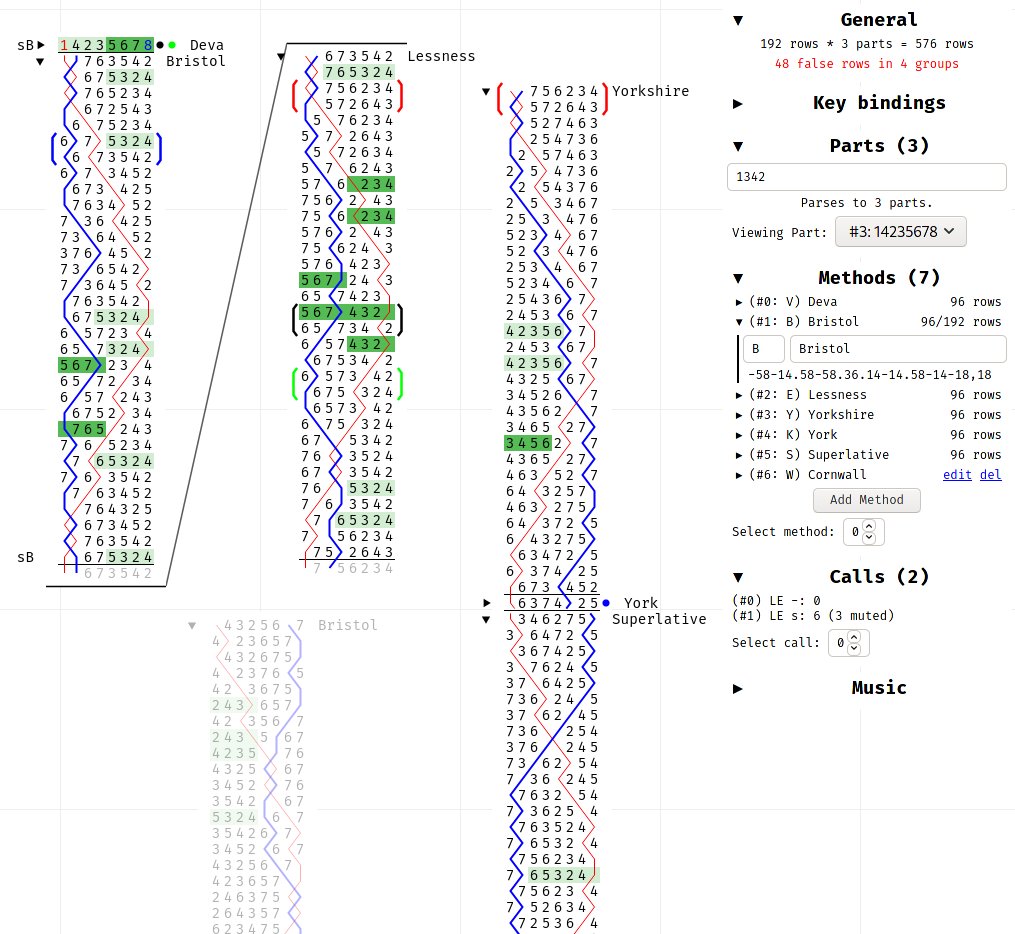
\includegraphics[width=0.8\textwidth]{current-screenshot-w-mute}
    \caption{Screenshot of Jigsaw, showing the folding UI and canvas
    display}\label{fig:cur-screenshot-2}
\end{figure}

\begin{figure}
    \centering
    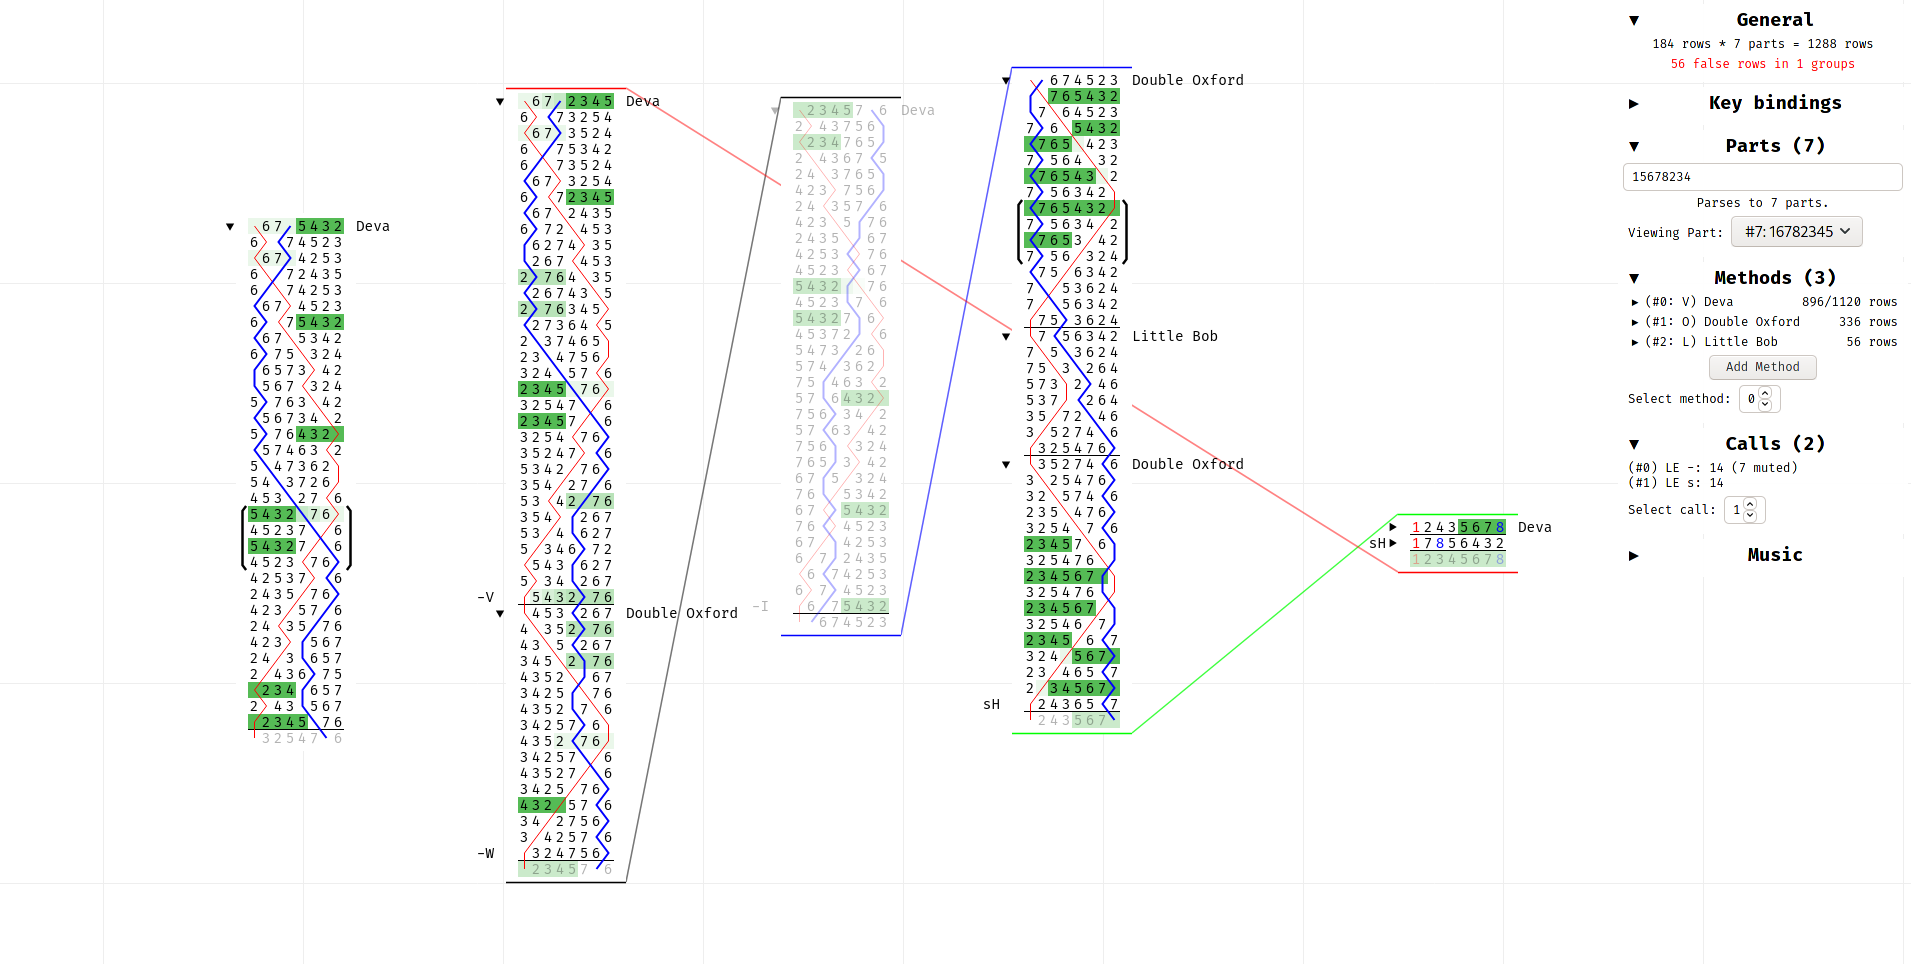
\includegraphics[width=\textwidth]{false-qp}
    \caption{Editing a Quarter Peal composition}\label{fig:cur-screenshot}
\end{figure}

Jigsaw is also designed to be used on a desktop with a 3-button mouse and keyboard, and optimises
for this use case.  All operations are bound to single keys with helpful mnemonics (e.g. \verb|a|
and \verb|A| to add to the composition), and these quickly become muscle memory and allow an
experienced user to quickly manipulate compositions.  For consistency, all operations are applied at
the location of the mouse cursor.  Editing speed is very important for software designed for
creative users, since work throughput is basically inversely proportional to iteration time --- the
more iterations are possible, the quicker and better the result will be.

Since most people use a mouse with their right hand, all operations are bound to keys on the left
side of the keyboard even if doing so requires worse mnemonics.  This means that every operation is
always instantly accessible to the user, maximising efficiency of editing and therefore improving
the user experience.

\subsection{Music Highlighting}

When music appears in a composition, the bells causing the music are highlighted green, giving an
an obvious visual indication of where the music is.

Additionally, non-musical rows can generate music in other parts of the composition, and in this
case the music is `onion-skinned' --- the more parts contain music, the darker the colour.  In
Figure~\ref{fig:multi-part-music}, for example, \row{4328} in the \nth{1}{st} lead is highlighted quite
densely because it generates \row{5432}, \row{6543}, etc.\ in other parts.  However, \row{8761} in
the \nth{4}{th} lead is highlighted very lightly because it only creates \row{4321} in the \nth{2}{nd}
lead.

\begin{figure}
    \centering
    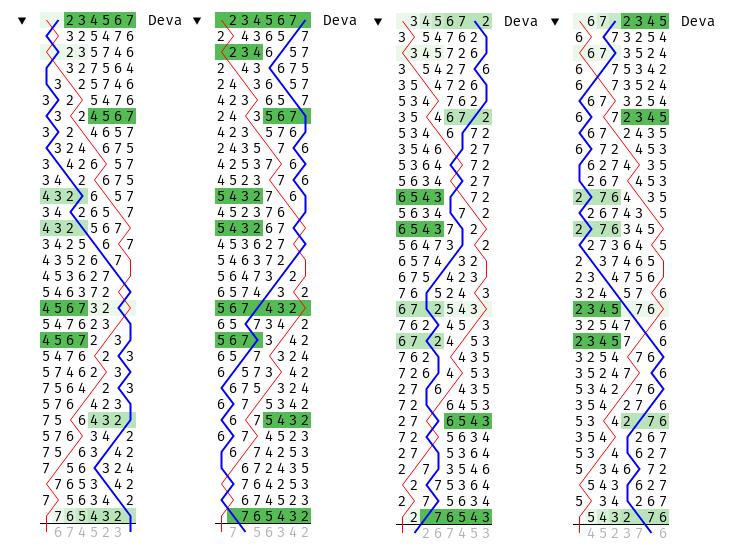
\includegraphics[width=0.6\textwidth]{multi-part-music-clean}
    \caption{The same lead in four different parts (rotating 2--8)}\label{fig:multi-part-music}
\end{figure}

\subsection{Falseness Display}

Falseness is visually communicated by marking groups of identical rows with the same coloured
brackets (see Figure~\ref{fig:falseness}).  As far as I know, this is the most efficient way of
visually communicating exact falseness.  The main drawbacks of this approach is that the number of
different groups can get very large causing Jigsaw to run out of easily differentiable colours.
Additionally, it is very reliant on colours which will likely be problematic for colour-blind
people.  A fix for this would be to add a switch to number the groups rather than just relying on
colour.

\begin{figure}
    \centering
    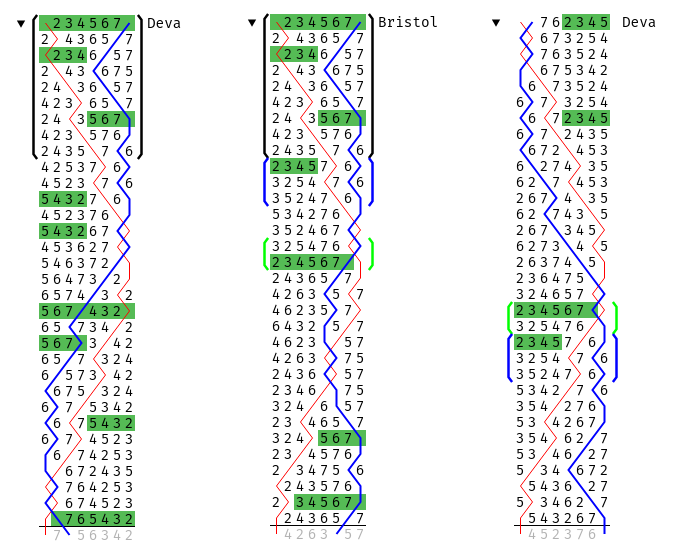
\includegraphics[width=0.5\textwidth]{falseness-clean}
    \caption{Leads which are false in 3 different ways}\label{fig:falseness}
\end{figure}

\subsection{Lead Folding}

To prevent the user from having to look at thousands of rows at the same time, Jigsaw allows leads
to be folded into a single row.  Jigsaw then converts falseness groups into dots next to the row
number (see Figure~\ref{fig:lead-folding}), and switches between lines and numbers for displaying
bells when necessary.

\begin{figure}
    \centering
    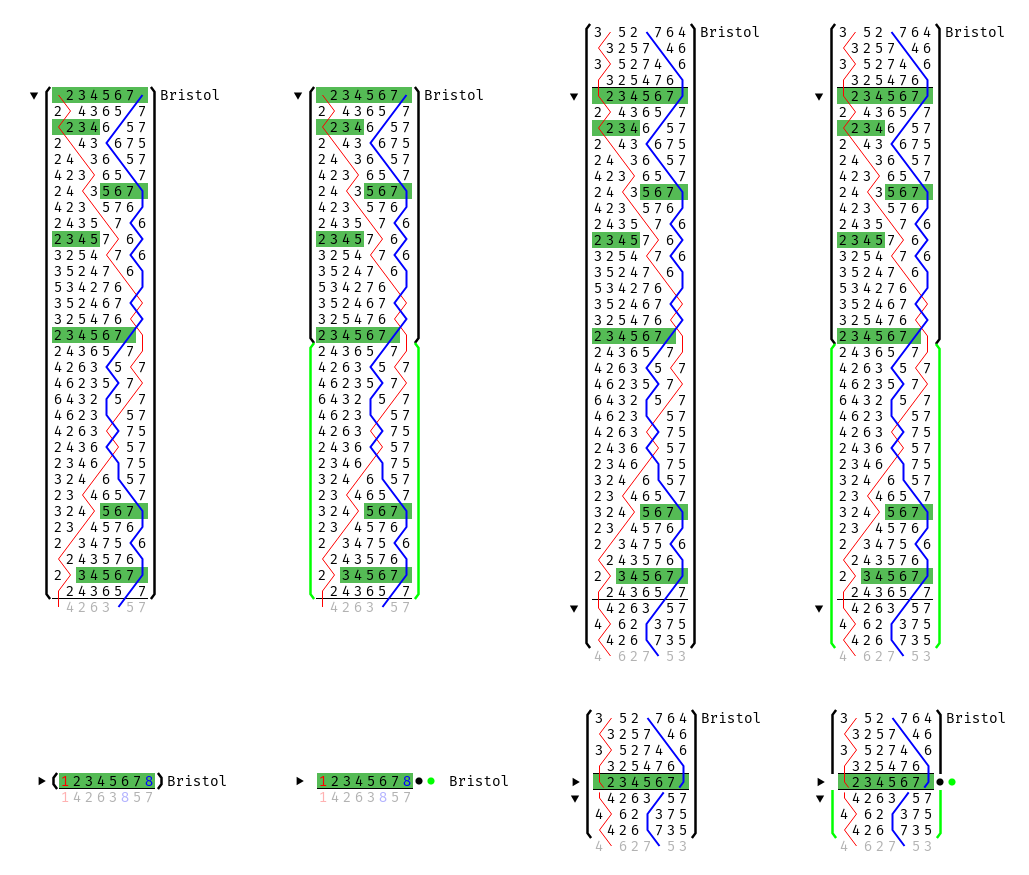
\includegraphics[width=0.78\textwidth]{folding-full}
    \caption{Unfolded (top) and folded (bottom) versions of the same lead.  Note the handling of
    falseness ranges and line segments.}\label{fig:lead-folding}
\end{figure}

\subsection{Linking Fragments}

Two fragments can be linked together if the leftover row of one is equal to the first row of the
other.  To represent this visually, Jigsaw draws a coloured line between the two (see
Figure~\ref{fig:linking}).  If multiple different sets of fragments link, then each group is
coloured separately (see Figure~\ref{fig:linking-insane}).

Hovering a line and pressing \verb|c| (for `connect') will join those fragments into one.  Note how
this operation does not change the rows contained in the composition.

\begin{figure}
    \centering
    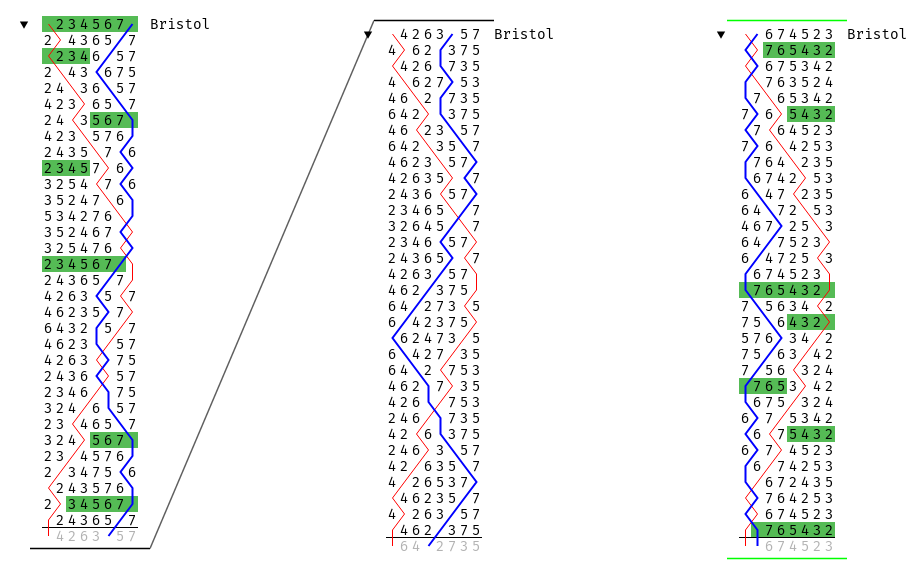
\includegraphics[width=0.8\textwidth]{linking-2}
    \caption{Two fragments which link together, and one that links to itself.}\label{fig:linking}
\end{figure}

\begin{figure}[h!]
    \centering
    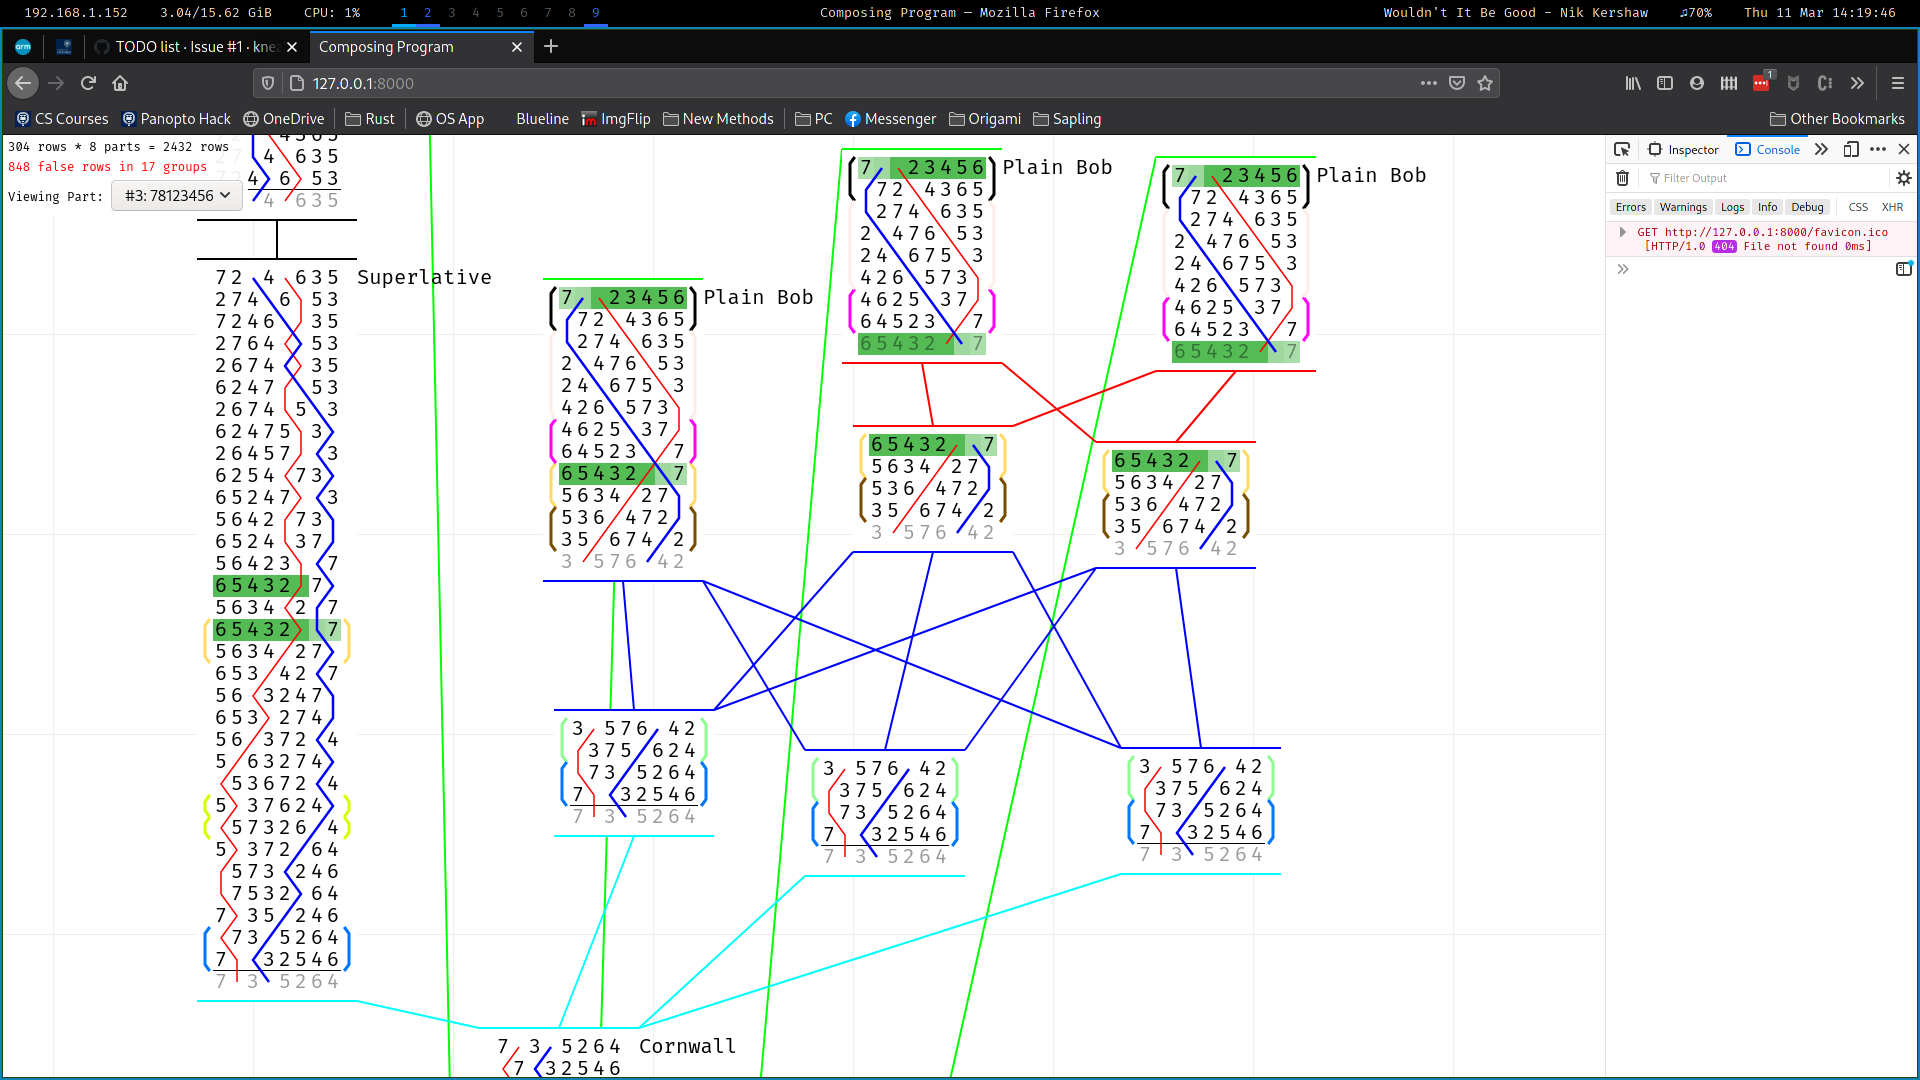
\includegraphics[width=\textwidth]{linking-insane}
    \caption{A lot of fragment links on one screen.}\label{fig:linking-insane}
\end{figure}



\pagebreak

\section{Implementation}

\subsection{Overview}

The code for Jigsaw is split into two main parts: two Rust libraries which together form a `server'
and `client' in the form of a web GUI.\@  The Rust code is compiled to WebAssembly, and exports an
API which allows the JavaScript client to make changes to the internal `model' and then request a
JSON serialisation of the information to display to the user.

This architecture plays to the strengths of both languages --- Rust provides fast and reliable data
manipulation whilst JavaScript, HTML and CSS provide a user-friendly cross-platform GUI.\@  The
binding and serialisation code is automatically generated at compile time using
\emph{wasm-bindgen}\footurl{https://github.com/rustwasm/wasm-bindgen} and
\emph{serde}\footurl{https://github.com/serde-rs/serde} to prevent human error.

\subsection{BellFrame}

Roughly half of the Rust code in the project is a cross-platform utility library for core data types
which are not specific to Jigsaw.  This provides safe and performant Rust data types for common
constructs related to change ringing (\verb|Row|, \verb|Bell|, \verb|Method|, \verb|Call|, etc.).
Its development and API design was motivated by Jigsaw but once its API is stable it will be
published to Rust's central package repository for general use.

The stable part of the API has good documentation and is well tested, and all data types only
provide public functions which preserve internal invariants and therefore obviate the need for
unnecessary checks.  It also provides `unsafe' versions of functions which remove runtime checks but
in rely on their caller to uphold the invariants.  Therefore, no undefined behaviour is possible if
the user only writes `safe' code.

Despite having no stable API, I have already built other projects on it.  In its own right, this
library is a valuable product of this project.

\subsubsection{Rows vs Permutations}

When writing BellFrame, I initially thought that the concept of rows and permutations were different
enough to warrant separate data types.  My thinking was that a \verb|Row| is a sequence of
\verb|Bell|s (plus some additional invariants), and a permutation can be thought of as a function of
type \verb|[a] -> [a]| which can permute sequences of any type.  Mathematically this feels like an
elegant separation, but using the library in earnest made me realise that the \verb|Perm| does not
pull its weight given its large overlap with the \verb|Row| type.  I would almost always use
\verb|Perm| only as an intermediate step to use one \verb|Row| to permute another.  Therefore, a few
months into the project the operations provided by \verb|Perm| were merged into \verb|Row|.

\subsection{Model-View-Presenter}

The code in the jigsaw library differentiates between the unique specification of a composition
(the \verb|Spec| type) and the information required to display it to the user (the
\verb|DerivedState| type).  The \verb|DerivedState| contains additional data like the music
locations, falseness and other annotations which are completely specified by the current
\verb|Spec| but necessary for displaying a composition.  Every change to the \verb|Spec| also causes
the \verb|DerivedState| to be updated before the changes can be displayed to the user.

Figure~\ref{fig:model-view-presenter} shows how Jigsaw's code maps to Model-View-Presenter.
Additionally, the Model-View-Presenter means that every edit passes completely through the model,
resulting in a data flow shown in Figure~\ref{fig:app-data-flow}.

\subsection{Specification vs Derived State}

The code in the jigsaw library differentiates between the unique specification of a composition
(the \verb|Spec| type) and the information required to display it to the user (the
\verb|DerivedState| type).  The \verb|DerivedState| contains additional data like the music
locations, falseness and other annotations.  That is completely specified by the contents of the
current \verb|Spec|, so every change to the \verb|Spec| must also cause the \verb|DerivedState| to
be updated before the changes can be displayed to the user.

In terms of Model-View-Presenter, the \verb|Spec| type is the Model whereas the \verb|DerivedState|
is the data sent from the Presenter to the View.

\begin{figure}
    \tikzstyle{blob} = [rectangle, rounded corners, minimum width=3cm, minimum height=1cm,text
    centered, draw=black]
    \tikzstyle{arrow} = [thick,->,>=stealth]

    \centering
    \begin{tikzpicture}[node distance=2cm]
        \node (view) [blob] {View (JavaScript)};
        \node (presenter) [blob, below of=view] {Presenter (\verb|Comp|)};
        \node (model) [blob, below of=presenter] {Model (\verb|Spec|)};

        \draw [arrow] ([xshift=-0.8cm]view.south) -- node [anchor=east] {Comp's API}
            ([xshift=-0.8cm]presenter.north);
        \draw [arrow] ([xshift=0.8cm]presenter.north) -- node [anchor=west]
            {Comp::ser\_derived\_state} ([xshift=0.8cm]view.south);

        \draw [arrow] ([xshift=-0.8cm]presenter.south) -- node [anchor=east] {Spec's API}
            ([xshift=-0.8cm]model.north);
        \draw [arrow] ([xshift=0.8cm]model.north) -- node [anchor=west]
            {DerivedState::from\_spec} ([xshift=0.8cm]presenter.south);
    \end{tikzpicture}
    \caption{Jigsaw's implementation of model-view-presenter}\label{fig:model-view-presenter}
\end{figure}

\begin{figure}
    \centering
    \tikzstyle{invis} = [minimum width=3cm, minimum height=1cm]
    \tikzstyle{title} = [minimum width=3cm, minimum height=1cm, text centered]
    \tikzstyle{blob} = [rectangle, rounded corners, minimum width=3cm, minimum height=0.9cm,text
        centered, draw=black]
    \tikzstyle{arrow} = [thick,->,>=stealth]


    \begin{tikzpicture}[node distance=1.7cm]
        \node (js) [title] {\textbf{JavaScript}};
        \node (rust) [title, xshift=5cm, right of=js] {\textbf{Rust}};

        \node (input) [blob, below of=js] {User input};
        \node (invis-1) [invis, below of=rust] {};

        \node (event) [blob, below of=input] {Event};
        \node (comp-api) [blob, below of=invis-1] {\verb|Comp::*| API};

        \node (invis-2) [invis, below of=event] {};
        \node (clone-spec) [blob, below of=comp-api] {Clone \verb|Spec|};

        \node (invis-3) [invis, below of=invis-2] {};
        \node (modify-spec) [blob, below of=clone-spec] {Modify new \verb|Spec|};

        \node (invis-4) [invis, below of=invis-3] {};
        \node (update-history) [blob, below of=modify-spec] {Update history};

        \node (invis-5) [invis, below of=invis-4] {};
        \node (rebuild-der-state) [blob, below of=update-history] {Rebuild \verb|DerivedState|};

        \node (sync-der-state) [blob, below of=invis-5] {\verb|sync_derived_state()|};
        \node (ser-der-state) [blob, below of=rebuild-der-state] {\verb|Comp::ser_derived_state|};

        \node (js-json-str) [blob, below of=sync-der-state] {JSON string};
        \node (rs-json-str) [blob, below of=ser-der-state] {JSON string};

        \node (js-der-state) [blob, below of=js-json-str] {\verb|derived_state| variable};

        \node (repaint) [blob, below of=js-der-state] {Repaint};

        \draw [arrow] (input) -- (event);
        \draw [arrow] (event) -- node [anchor=south] {API call} (comp-api);
        \draw [arrow] (event) |- node [anchor=west, pos=0.1] {undo/redo} (update-history);
        \draw [arrow] (comp-api) -- (clone-spec);
        \draw [arrow] (clone-spec) -- (modify-spec);
        \draw [arrow] (modify-spec) -- (update-history);
        \draw [arrow] (update-history) -- (rebuild-der-state);
        \draw [arrow] (rebuild-der-state) -| node [anchor=south, pos=0.25] {return} (sync-der-state);
        \draw [arrow] (sync-der-state) -- node [anchor=south] {API call} (ser-der-state);
        \draw [arrow] (ser-der-state) -- node [anchor=west] {\emph{serde}} (rs-json-str);
        \draw [arrow] (rs-json-str) -- node [anchor=south] {return} (js-json-str);
        \draw [arrow] (js-json-str) -- node [anchor=west] {deserialise} (js-der-state);
        \draw [arrow] (js-der-state) -- (repaint);
    \end{tikzpicture}
    \caption{The data flow of user's changes}\label{fig:app-data-flow}
\end{figure}

\subsection{Undo History}

Jigsaw uses the `immutable data structure' method of storing undo history, where the history is a
sequence of fully defined states (as opposed to an event system where the history is a sequence of
modifications).  Therefore, the undo history is simply a list of \verb|Spec| types along with an
index referring to the `current' \verb|Spec| being displayed on the screen.

In order to prevent unnecessary duplication of data, the internal data of the \verb|Spec| type is
always stored behind reference-counted pointers.  Therefore, cloning a \verb|Spec| adds one to the
reference count rather than cloning the backing data.  In Rust, reference-counted pointers are
always immutable so in order to modify some part of the data, we have to clone the part using
\verb|Rc::make_mut| provided by the standard library.  Rust checks this at compile-time and will
reject code which tries to modify shared data without first cloning it.

This approach works excellently, and allows Jigsaw to fully update the display without adding steps
to the undo history.  This gives the user instant feedback when transposing fragments.

\subsubsection{Passing Data Between Rust and JavaScript}

Even with \emph{wasm-bindgen} providing binding code, all data types that can be sent over the
language interface are limited to flat structures with no references.  This is unfortunate, since
\verb|DerivedState| has 4 layers of references (\verb|DerivedState| $\to$ \verb|DerivedFrag| $\to$
\verb|DisplayRow| $\to$ \verb|Row| $\to$ \verb|Bell|), all of which is required to render each
frame.  Therefore, it is not possible to simply return the \verb|DerivedState| from Rust into
JavaScript, and another strategy is required.

Initially, I did not want JavaScript and Rust to hold their own copies of \verb|DerivedState|,
because then there would be two potentially divergent sources of the truth (causing bugs which would
be extremely hard to fix).  Additionally, I wanted to limit the complexity handled by the JavaScript
code (due to its inferior performance and maintainability) so it felt natural for Rust to handle all
the state and then expose a simple API to JavaScript to read the data.

The original API was a flat set of getter functions, looking like Figure~\ref{fig:initial-api}.
This worked fine for a while but as the complexity of \verb|DerivedState| grew, the number of
exported functions exploded and refactoring the API became unnecessarily challenging.  Also, every
WebAssembly function call takes a non-trivial amount of time and this flat API encourages huge
numbers of calls in each frame which started causing performance issues.  It is also worth noting
that the \verb|DerivedState| only changes when the user changes the composition, but is needed every
time the UI is painted.

\begin{figure}
    \begin{verbatim}
/// Get the number of fragments
fn get_num_frags() -> usize { ... }

/// Get the number of rows in the fragment at a given index
fn get_frag_length(frag_index: usize) -> usize { ... }

/// Get the bell at a given location
fn get_row(
    frag_index: usize,
    row_index: usize,
    bell_index: usize
) -> Bell { ... }
    \end{verbatim}
    \caption{Initial getter API design}\label{fig:initial-api}
\end{figure}

Eventually, I settled on the strategy that Jigsaw currently uses:  to pass the entire
\verb|DerivedState| structure as a JSON string after each edit.  JavaScript then parses and caches
the resulting object which it reads from when drawing each frame.  This turned out to work really
well --- almost no WebAssembly calls are made during each frame, the `getter' API is reduced to a
single function and long-term divergence is still impossible because JavaScript completely
overwrites its copy of the \verb|DerivedState| each time the composition updates.

The serialisation code is generated at compile-time using
\emph{serde}\footurl{https://github.com/serde-rs/serde}, removing the possibility for human error.
Therefore, the data in JavaScript and Rust will always have the same structure, making the whole
code base much easier to read and refactor.



\pagebreak

\section{Assessment and Analysis}

\subsection{Jigsaw}

\subsubsection{Overview}

I think that Jigsaw is a successful prototype and has potential to be built into a  feature-complete
application, which I now plan to do. I demonstrated it to several other composers during development
for feedback on the design.  This was positive, they all thought it looked very promising, but
identified a number of minor issues that would allow it to be more useful in finished form.

In order to decide on the success of the project, I will rank it against the design goals set out in
Section~\ref{sec:design-goals}.

\subsubsection{Ease of Use \& Visual}

Firstly, building Jigsaw as a single static page means it requires no installation to use.  The
design of an infinite canvas plus a folding sidebar feels very natural and intuitive to use.

A large amount of effort went into making sure that GUI is visually crisp and responsive.  This
goes as far as rounding all coordinates to the nearest pixel to prevent fuzzy boundaries and
erroneous gaps, as well as doing the same for line rendering.  Attention to detail like this makes
the experience of using Jigsaw feel very smooth and polished.

All actions are currently bound to easily accessible keys which means that editing compositions
quickly becomes muscle memory for experienced users, but feels unintuitive to beginners because
there is no indicator of what actions are available in a given location.  In a future development of
Jigsaw I will consider adding a contextual right-click menu.  Such a menu can even show the key
bindings to help beginners learn them.

\subsubsection{Completeness}

Jigsaw's internal representation is complete, but the current user interface is not.  In other
words, Jigsaw is internally able to represent a strict superset of compositions which are considered
change ringing, but the prototype GUI means that the user is unable to express some very obscure
states which are technically considered change ringing.  For perhaps 99\% of use cases, Jigsaw's
user interface is complete enough that most users would not notice.

\subsubsection{Incremental}

Jigsaw is completely built around being incremental.  It also does its best to preserve `continuity'
of operations --- that is, a small operation should cause a small change to the composition's rows.
Some operations like splitting and joining fragments only change the structure of the composition,
and not the output rows.

\subsubsection{Instant}

Due to the internal architecture, the composition is always fully annotated.  Whenever the user
causes an update, the entire state of the display is recalculated then cached for repainting.
Therefore, it simply is not possible for any part of the changes to lag behind because the full UI
state is simultaneously recalculated after every change.

This does, however, mean that Jigsaw is extremely dependent on the efficiency of this update
pipeline.  Luckily, Rust and WebAssembly work extremely well in this regard since the
pipeline is fast enough to reliably feel instant, even for large compositions.  I have not done any
specific optimisations, but I have been mindful of high-level performance when writing the code
--- the algorithms are all $O(n \log n)$ in the number of bells in the composition, although the
link detection is $O(n^2)$ in the number of fragments.  This means that Jigsaw is far from its
potential performance ceiling, allowing for straightforward optimisations in case the UI stops
feeling instant in the future.

Whilst stress testing Jigsaw, I discovered that this delay becomes noticeable at around 35,000
$\times$ 8 = 280,000 bells (see Figure~\ref{fig:stress-test}).  Since 99.7\%\footnote{44,551 out of
44,683 compositions on Composition Library have this property, as of \nth{23}{rd} of May 2021.} of
compositions have at most 10,000 rows each of 16 bells (making 160,000 bells total) I think that the
performance is adequate.

The longest piece of ringing ever rung contains 72,000 $\times$ 6 = 432,000 bells, which would
challenge the performance of the current implementation.  In reality, the composition for this was
split into many separate pieces to ease memorability so I doubt anyone would want to work on a
composition of this size in full.  However, I would like Jigsaw to eventually support huge
compositions and there is plenty of opportunity to optimise --- for example, the pipeline does no
caching or re-use of heap allocations so the code generates huge numbers of needless allocations
during each pipeline run.

Additionally, BellFrame contains the \verb|SimdRow| type which uses SIMD instructions
(specifically \verb|pshufb|) to perform row permutations in a single clock cycle, which usually
increases performance by at least an order of magnitude.  Furthermore, \verb|SimdRow| is also
constant size, removing heap allocations.  In return for this huge performance improvement,
\verb|SimdRow| has a fixed limit of 16 bells which requires any code to dynamically fall back on the
heap-allocated \verb|Row| when required, significantly increasing the complexity and potentially
creating obscure bugs.  Finally, SIMD is not supported in mainstream WebAssembly yet so Jigsaw will
have to wait before \verb|SimdRow| is an option.

\begin{figure}
    \centering
    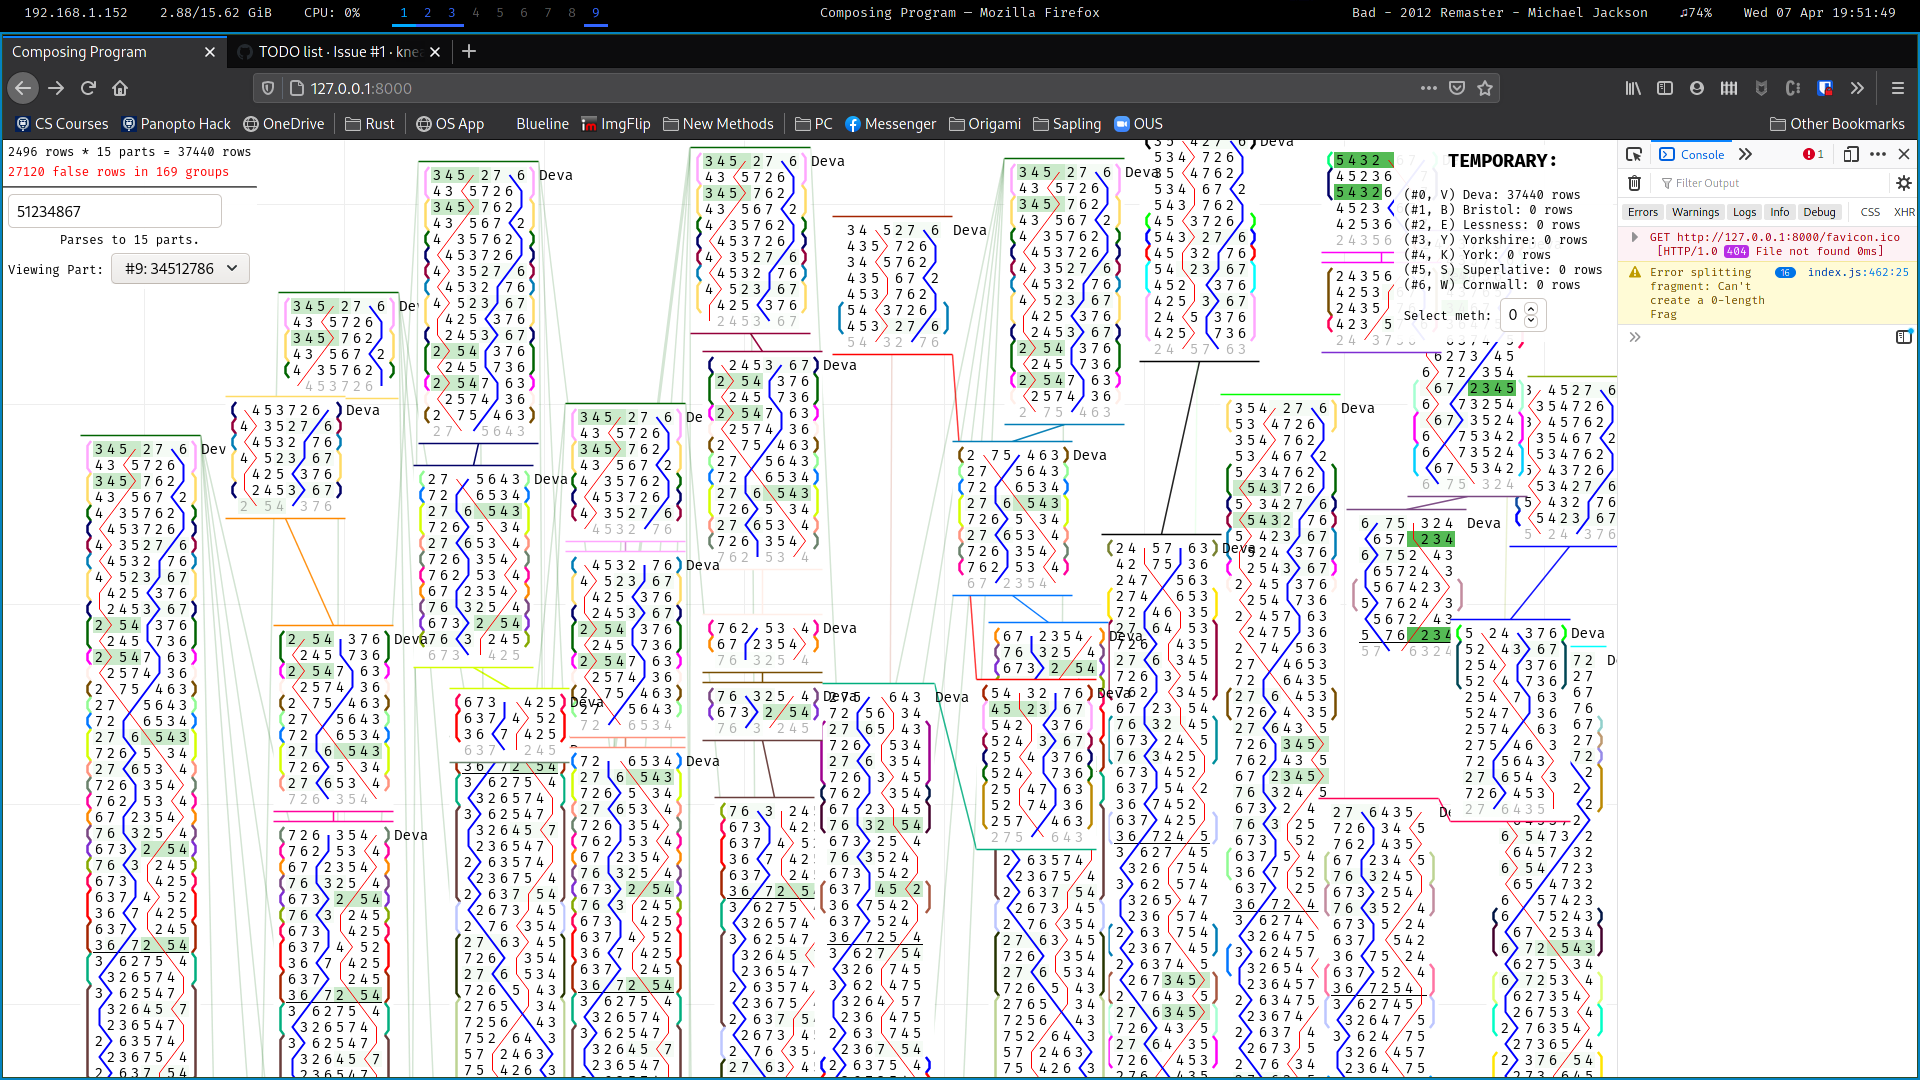
\includegraphics[width=\textwidth]{stress-test}
    \caption{Stress testing Jigsaw (the GUI has since changed, but the pipeline has
    not).}\label{fig:stress-test}
\end{figure}

\subsection{Final Statistics}

As of writing this report, Jigsaw's GitHub repository has 275 commits and contains 5,736 source
lines of code (including 4,233 of Rust, 1,033 of JavaScript, 240 of HTML, 114 of CSS and 85 of
Python for the build script).  Including comments and blanks, this increases to 7,556 lines.



\pagebreak

\section{Conclusion}

This project set out to create a prototype for an application to aid composers of church bell
ringing.  A general design goal was set, and this was broken down into five specific requirements.
The resulting tool, Jigsaw has met all of the five requirements and its usefulness has been
validated by beta-testing and feedback from experienced composers. Jigsaw's combination of intuitive
graphical interface and efficient implementation has proved highly effective.

The reusable utility library on which Jigsaw is built (named BellFrame) is also a significant
contribution to composition which others will be able to benefit from.

In the next stage of development I would propose to take the prototype and address the minor issues
identified in beta-testing and further improve usability, for example with a right-click menu. I
would use a more complete testing process --- automated testing of the code to improve reliability
and user testing to refine the user experience.  This will ensure that Jigsaw is consistently
robust in a wide range of use cases.

Creation of this prototype has been a valuable learning experience.  If I were to do a similar
project again I would be more careful about which order features should be designed and implemented.
For example, retrofitting lead folding was unnecessarily difficult and this extra complexity would
be avoided had I implemented it earlier.  When building a production application, I would place a
much heavier emphasis on stability and automated testing than I did for Jigsaw.  However, for
prototypes like Jigsaw, the rapid iteration means that tests are often invalidated shortly after
their creation.

Finally, I would like to acknowledge the guidance of my project supervisor, Dr Geraint Jones and the
composers --- past and present --- who inspired me to create this tool.



\pagebreak

\section{Glossary of Change Ringing Terms}\label{sec:glossary}

\paragraph{Stage:} The number of bells which the composition uses.  This is not necessarily the
number of bells used to ring a given composition, but for the purposes of this project the
distinction is not relevant.

\paragraph{Row:} A sequence of bells which forms a permutation.  Rows are the fundamental building
blocks of compositions.  The words `change' and `row' are often used interchangeably (hence the name
`Change Ringing'), but to avoid confusion I will always use `row' in this report.

\paragraph{Composition:} An ordered sequence of rows which tell ringers in which order the bells
should be rung.

\paragraph{Truth:} For the purposes of this project, a composition is \emph{`true'} if all the rows
are unique, otherwise it is \emph{`false'}.  This is the single most important property of a
composition, since any performance of a `false' composition is considered invalid.

\paragraph{Method:} A short, usually symmetrical, pattern that is repeated throughout a composition
with small and well-defined modifications (known as `calls').  This is the key to how human ringers
can ring over 5000 rows worth of composition without any memory aid --- in reality, they memorise
the method(s) and one `conductor' memorises the pattern of calls and calls them in the right places
for the other ringers to obey.  It is usually the job of the composer to make sure that the call
sequence is predictable and easy to memorise, whilst preserving other valued properties.

\paragraph{Lead:} A single instance of the repeating pattern of a method.

\paragraph{Rounds:} A special row with all the bells in ascending order of number (written
\verb|123456...|).  All compositions must start and finish in rounds.

\end{document}
